% --
% wavenets

\section{Experiments on Wavenets}\label{exp_wavenet}
\thesisStateReady
Very few experiments were performed on the Wavenet architecture shown in \rsec{nn_arch_wavenet}, because of its complex model structure and heavy computational footprint.
It is taking much time and energy consumption for few training epochs, further the results on the accuracy of classifying speech commands were really bad.
This architecture is therefore left for future research.
Nevertheless the best performing model is presented here, which was trained with 500 examples per each one of the L12 labels, 100 epochs, a learning rate of $0.001$ for 10 epochs and a changing to a learning rate of $0.0001$ and a usual batch size of 32.
The accuracy score for the training and the confusion matrix is shown in \rfig{exp_wavenet_acc} and \rfig{exp_wavenet_confusion}.
The best achieved accuracy on the test set was merely \SI{38.83}{\percent}.
\begin{figure}[!ht]
  \centering
  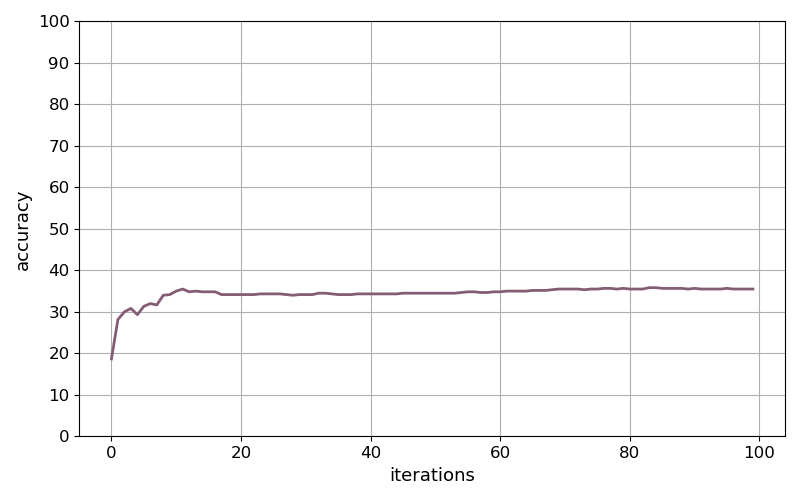
\includegraphics[width=0.45\textwidth]{./5_exp/figs/exp_wavenet_acc}
  \caption{Accuracies on the validation set during the training of the Wavenet model with classification extension.}
  \label{fig:exp_wavenet_acc}
\end{figure}
\begin{figure}[!ht]
  \centering
  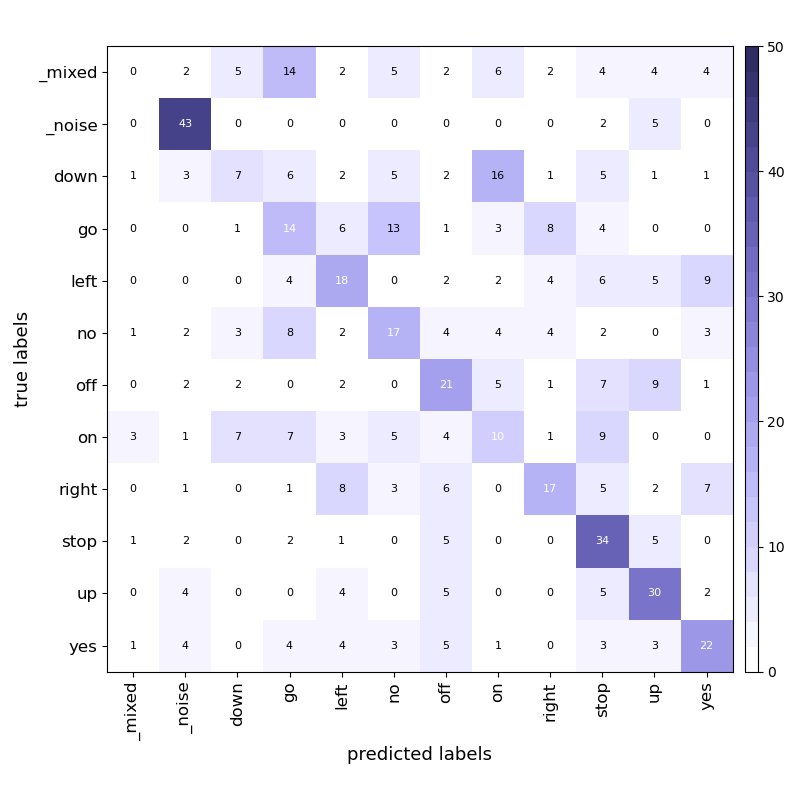
\includegraphics[width=0.45\textwidth]{./5_exp/figs/exp_wavenet_confusion_test}
  \caption{Confusion matrix of the test set evaluated on the trained Wavenet model.}
  \label{fig:exp_wavenet_confusion}
\end{figure}
\FloatBarrier
\noindent